\subsection{Branch Coverage}\label{sec:branch_coverage}
\begin{table*}[]
    \centering
    \caption{Branch coverage of $\ourtool$ and four baselines across three consecutive releases for each benchmark.}
    \label{tab:coverage_main}
    \resizebox{\textwidth}{!}{%
    \setlength{\tabcolsep}{3pt}
    \begin{tabular}{l|l|rrrrr||l|l|rrrrr||l|l|rrrrr}
    \toprule \midrule
    \multicolumn{1}{c|}{Program} & \multicolumn{1}{c|}{Version} & \multicolumn{1}{c|}{$\ourtool$}            & \multicolumn{1}{c|}{$\default$}    & \multicolumn{1}{c|}{$\rerun$}   & \multicolumn{1}{c|}{$\seeding$} & \multicolumn{1}{c||}{$\naive$} & \multicolumn{1}{c|}{Program} & \multicolumn{1}{c|}{Version} & \multicolumn{1}{c|}{$\ourtool$}            & \multicolumn{1}{c|}{$\default$}    & \multicolumn{1}{c|}{$\rerun$}   & \multicolumn{1}{c|}{$\seeding$} & \multicolumn{1}{c||}{$\naive$} & \multicolumn{1}{c|}{Program} & \multicolumn{1}{c|}{Version} & \multicolumn{1}{c|}{$\ourtool$}            & \multicolumn{1}{c|}{$\default$}    & \multicolumn{1}{c|}{$\rerun$}   & \multicolumn{1}{c|}{$\seeding$} & \multicolumn{1}{c}{$\naive$} \\ \midrule \midrule
    \multirow{3}{*}{bison}       & 3.6                          & \multicolumn{5}{c||}{928.2}                                                                                                                                      & \multirow{3}{*}{gawk}        & 5.3.0                        & \multicolumn{5}{c||}{2,357.4}                                                                                                                                    & \multirow{3}{*}{objcopy}     & 2.43                         & \multicolumn{5}{c}{252.0}                                                                                                                                      \\ \cmidrule(lr){2-7} \cmidrule(lr){9-14} \cmidrule{16-21} 
                                 & 3.7                          & \multicolumn{1}{r|}{\textbf{1,271.0}} & \multicolumn{1}{r|}{1,064.8} & \multicolumn{1}{r|}{1,092.0} & \multicolumn{1}{r|}{991.6}   & 936.6                      &                              & 5.3.1                        & \multicolumn{1}{r|}{\textbf{3,450.2}} & \multicolumn{1}{r|}{2,153.6} & \multicolumn{1}{r|}{2,401.4} & \multicolumn{1}{r|}{3,017.0} & 2,906.8                    &                              & 2.44                         & \multicolumn{1}{r|}{\textbf{539.8}}   & \multicolumn{1}{r|}{385.0}   & \multicolumn{1}{r|}{394.4}   & \multicolumn{1}{r|}{529.6}   & 507.8                     \\ \cmidrule(lr){2-7} \cmidrule(lr){9-14} \cmidrule{16-21} 
                                 & 3.8                          & \multicolumn{1}{r|}{\textbf{1,295.4}} & \multicolumn{1}{r|}{886.2}   & \multicolumn{1}{r|}{1,097.4} & \multicolumn{1}{r|}{1,005.4} & 808.6                      &                              & 5.3.2                        & \multicolumn{1}{r|}{\textbf{3,546.0}} & \multicolumn{1}{r|}{2,311.2} & \multicolumn{1}{r|}{2,580.0} & \multicolumn{1}{r|}{3,049.0} & 2,883.6                    &                              & 2.45                         & \multicolumn{1}{r|}{\textbf{550.4}}   & \multicolumn{1}{r|}{352.2}   & \multicolumn{1}{r|}{406.4}   & \multicolumn{1}{r|}{533.2}   & 513.6                     \\ \midrule
    \multirow{3}{*}{csplit}      & 9.7                          & \multicolumn{5}{c||}{445.8}                                                                                                                                      & \multirow{3}{*}{grep}        & 3.10                         & \multicolumn{5}{c||}{1,067.6}                                                                                                                                    & \multirow{3}{*}{objdump}     & 2.43                         & \multicolumn{5}{c}{278.6}                                                                                                                                      \\ \cmidrule(lr){2-7} \cmidrule(lr){9-14} \cmidrule{16-21} 
                                 & 9.8                          & \multicolumn{1}{r|}{\textbf{516.8}}   & \multicolumn{1}{r|}{415.0}   & \multicolumn{1}{r|}{425.4}   & \multicolumn{1}{r|}{454.8}   & 443.6                      &                              & 3.11                         & \multicolumn{1}{r|}{\textbf{2,166.8}} & \multicolumn{1}{r|}{1,020.4} & \multicolumn{1}{r|}{1,120.6} & \multicolumn{1}{r|}{1,046.2} & 1,074.0                    &                              & 2.44                         & \multicolumn{1}{r|}{\textbf{469.0}}   & \multicolumn{1}{r|}{194.4}   & \multicolumn{1}{r|}{215.6}   & \multicolumn{1}{r|}{427.4}   & 213.8                     \\ \cmidrule(lr){2-7} \cmidrule(lr){9-14} \cmidrule{16-21} 
                                 & 9.9                          & \multicolumn{1}{r|}{\textbf{521.4}}   & \multicolumn{1}{r|}{414.4}   & \multicolumn{1}{r|}{429.6}   & \multicolumn{1}{r|}{453.8}   & 442.4                      &                              & 3.12                         & \multicolumn{1}{r|}{\textbf{2,229.0}} & \multicolumn{1}{r|}{1,209.0} & \multicolumn{1}{r|}{1,338.4} & \multicolumn{1}{r|}{1,155.2} & 1,337.4                    &                              & 2.45                         & \multicolumn{1}{r|}{\textbf{481.0}}   & \multicolumn{1}{r|}{190.6}   & \multicolumn{1}{r|}{225.4}   & \multicolumn{1}{r|}{464.8}   & 204.8                     \\ \midrule
    \multirow{3}{*}{diff}        & 3.10                         & \multicolumn{5}{c||}{520.6}                                                                                                                                      & \multirow{3}{*}{ls}          & 9.7                          & \multicolumn{5}{c||}{1,402.6}                                                                                                                                    & \multirow{3}{*}{patch}       & 2.6                          & \multicolumn{5}{c}{395.0}                                                                                                                                      \\ \cmidrule(lr){2-7} \cmidrule(lr){9-14} \cmidrule{16-21} 
                                 & 3.11                         & \multicolumn{1}{r|}{\textbf{575.0}}   & \multicolumn{1}{r|}{434.2}   & \multicolumn{1}{r|}{541.4}   & \multicolumn{1}{r|}{569.0}   & 469.4                      &                              & 9.8                          & \multicolumn{1}{r|}{\textbf{1,650.8}} & \multicolumn{1}{r|}{1,461.6} & \multicolumn{1}{r|}{1,487.0} & \multicolumn{1}{r|}{1,460.4} & 1,452.0                    &                              & 2.7                          & \multicolumn{1}{r|}{\textbf{859.2}}   & \multicolumn{1}{r|}{457.6}   & \multicolumn{1}{r|}{626.6}   & \multicolumn{1}{r|}{765.2}   & 731.2                     \\ \cmidrule(lr){2-7} \cmidrule(lr){9-14} \cmidrule{16-21} 
                                 & 3.12                         & \multicolumn{1}{r|}{\textbf{596.8}}   & \multicolumn{1}{r|}{425.2}   & \multicolumn{1}{r|}{548.8}   & \multicolumn{1}{r|}{574.0}   & 410.6                      &                              & 9.9                          & \multicolumn{1}{r|}{\textbf{1,693.4}} & \multicolumn{1}{r|}{1,462.8} & \multicolumn{1}{r|}{1,517.2} & \multicolumn{1}{r|}{1,462.2} & 1,407.4                    &                              & 2.8                          & \multicolumn{1}{r|}{\textbf{877.4}}   & \multicolumn{1}{r|}{504.0}   & \multicolumn{1}{r|}{654.8}   & \multicolumn{1}{r|}{774.0}   & 744.8                     \\ \midrule
    \multirow{3}{*}{du}          & 9.7                          & \multicolumn{5}{c||}{980.2}                                                                                                                                      & \multirow{3}{*}{m4}          & 1.4.18                       & \multicolumn{5}{c||}{564.4}                                                                                                                                      & \multirow{3}{*}{sqlite}      & 3.51.0                       & \multicolumn{5}{c}{4,402.8}                                                                                                                                    \\ \cmidrule(lr){2-7} \cmidrule(lr){9-14} \cmidrule{16-21} 
                                 & 9.8                          & \multicolumn{1}{r|}{\textbf{1,136.2}} & \multicolumn{1}{r|}{961.0}   & \multicolumn{1}{r|}{988.8}   & \multicolumn{1}{r|}{1,040.2} & 979.4                      &                              & 1.4.19                       & \multicolumn{1}{r|}{\textbf{636.2}}   & \multicolumn{1}{r|}{341.4}   & \multicolumn{1}{r|}{576.6}   & \multicolumn{1}{r|}{279.6}   & 335.0                      &                              & 3.51.1                       & \multicolumn{1}{r|}{\textbf{5,288.4}} & \multicolumn{1}{r|}{4,551.6} & \multicolumn{1}{r|}{4,927.6} & \multicolumn{1}{r|}{5,041.2} & 4,538.8                   \\ \cmidrule(lr){2-7} \cmidrule(lr){9-14} \cmidrule{16-21} 
                                 & 9.9                          & \multicolumn{1}{r|}{\textbf{1,146.4}} & \multicolumn{1}{r|}{945.6}   & \multicolumn{1}{r|}{1,004.0} & \multicolumn{1}{r|}{1,047.4} & 992.2                      &                              & 1.4.20                       & \multicolumn{1}{r|}{\textbf{661.8}}   & \multicolumn{1}{r|}{468.0}   & \multicolumn{1}{r|}{584.8}   & \multicolumn{1}{r|}{371.2}   & 444.2                      &                              & 3.51.2                       & \multicolumn{1}{r|}{\textbf{5,674.0}} & \multicolumn{1}{r|}{4,580.2} & \multicolumn{1}{r|}{5,057.2} & \multicolumn{1}{r|}{5,532.2} & 4,574.4                   \\ \midrule
    \multirow{3}{*}{find}        & 4.8.0                        & \multicolumn{5}{c||}{1,123.6}                                                                                                                                    & \multirow{3}{*}{make}        & 4.2                          & \multicolumn{5}{c||}{1,386.0}                                                                                                                                    & \multirow{3}{*}{xorriso}     & 1.5.2                        & \multicolumn{5}{c}{2,161.4}                                                                                                                                    \\ \cmidrule(lr){2-7} \cmidrule(lr){9-14} \cmidrule{16-21} 
                                 & 4.9.0                        & \multicolumn{1}{r|}{\textbf{1,635.8}} & \multicolumn{1}{r|}{1,116.6} & \multicolumn{1}{r|}{1,147.4} & \multicolumn{1}{r|}{1,357.8} & 1,533.4                    &                              & 4.3                          & \multicolumn{1}{r|}{\textbf{1,912.6}} & \multicolumn{1}{r|}{1,410.2} & \multicolumn{1}{r|}{1,437.6} & \multicolumn{1}{r|}{1,414.4} & 1,458.0                    &                              & 1.5.4                        & \multicolumn{1}{r|}{\textbf{2,880.0}} & \multicolumn{1}{r|}{2,141.6} & \multicolumn{1}{r|}{2,208.8} & \multicolumn{1}{r|}{2,366.6} & 1,909.0                   \\ \cmidrule(lr){2-7} \cmidrule(lr){9-14} \cmidrule{16-21} 
                                 & 4.10.0                       & \multicolumn{1}{r|}{\textbf{1,658.4}} & \multicolumn{1}{r|}{1,096.4} & \multicolumn{1}{r|}{1,171.2} & \multicolumn{1}{r|}{1,506.6} & 1,524.4                    &                              & 4.4                          & \multicolumn{1}{r|}{\textbf{2,027.2}} & \multicolumn{1}{r|}{1,482.6} & \multicolumn{1}{r|}{1,496.6} & \multicolumn{1}{r|}{1,403.0} & 1,503.0                    &                              & 1.5.6                        & \multicolumn{1}{r|}{\textbf{3,194.0}} & \multicolumn{1}{r|}{2,009.0} & \multicolumn{1}{r|}{2,235.0} & \multicolumn{1}{r|}{2,420.2} & 1,987.8                   \\ \midrule \bottomrule
    \end{tabular}%
    }
\end{table*}



\iffalse
\begin{table*}[]
    \centering
    \caption{Branch coverage of $\ourtool$ and four baselines across three consecutive releases for each benchmark.}
    \label{tab:coverage_main}
    \resizebox{0.8\textwidth}{!}{%
    \setlength{\tabcolsep}{3pt}
    \begin{tabular}{l|l|rrrrr||l|l|rrrrr}
    \toprule \midrule
    Program                 & Version & \multicolumn{1}{c|}{$\ourtool$}   & \multicolumn{1}{c|}{$\default$}    & \multicolumn{1}{c|}{$\rerun$}   & \multicolumn{1}{c|}{$\seeding$}    & \multicolumn{1}{c||}{$\naive$} & Program                  & Version & \multicolumn{1}{c|}{$\ourtool$}    & \multicolumn{1}{c|}{$\default$}     & \multicolumn{1}{c|}{$\rerun$}    & \multicolumn{1}{c|}{$\seeding$}     & \multicolumn{1}{c}{$\naive$} \\ \midrule \midrule
    \multirow{3}{*}{bison}  & 3.6     & \multicolumn{5}{c||}{928.2}                                                                                                                             & \multirow{3}{*}{m4}      & 1.4.18  & \multicolumn{5}{c}{564.4}                                                                                                                                 \\ \cmidrule(lr){2-7} \cmidrule{9-14} 
                            & 3.7     & \multicolumn{1}{r|}{\textbf{1,271.0}} & \multicolumn{1}{r|}{1,064.8} & \multicolumn{1}{r|}{1,092.0} & \multicolumn{1}{r|}{991.6}   & 936.6                      &                          & 1.4.19  & \multicolumn{1}{r|}{\textbf{636.2}}    & \multicolumn{1}{r|}{341.4}    & \multicolumn{1}{r|}{576.6}    & \multicolumn{1}{r|}{279.6}    & 335.0                     \\ \cmidrule(lr){2-7} \cmidrule{9-14} 
                            & 3.8     & \multicolumn{1}{r|}{\textbf{1,295.4}} & \multicolumn{1}{r|}{886.2}   & \multicolumn{1}{r|}{1,097.4} & \multicolumn{1}{r|}{1,005.4} & 808.6                      &                          & 1.4.20  & \multicolumn{1}{r|}{\textbf{661.8}}    & \multicolumn{1}{r|}{468.0}    & \multicolumn{1}{r|}{584.8}    & \multicolumn{1}{r|}{371.2}    & 444.2                     \\ \midrule
    \multirow{3}{*}{csplit} & 9.7     & \multicolumn{5}{c||}{445.8}                                                                                                                             & \multirow{3}{*}{make}    & 4.2     & \multicolumn{5}{c}{1,386.0}                                                                                                                               \\ \cmidrule(lr){2-7} \cmidrule{9-14} 
                            & 9.8     & \multicolumn{1}{r|}{\textbf{516.8}}   & \multicolumn{1}{r|}{415.0}   & \multicolumn{1}{r|}{425.4}   & \multicolumn{1}{r|}{454.8}   & 443.6                      &                          & 4.3     & \multicolumn{1}{r|}{\textbf{1,912.6}}  & \multicolumn{1}{r|}{1,410.2}  & \multicolumn{1}{r|}{1,437.6}  & \multicolumn{1}{r|}{1,414.4}  & 1,458.0                   \\ \cmidrule(lr){2-7} \cmidrule{9-14} 
                            & 9.9     & \multicolumn{1}{r|}{\textbf{521.4}}   & \multicolumn{1}{r|}{414.4}   & \multicolumn{1}{r|}{429.6}   & \multicolumn{1}{r|}{453.8}   & 442.4                      &                          & 4.4     & \multicolumn{1}{r|}{\textbf{2,027.2}}  & \multicolumn{1}{r|}{1,482.6}  & \multicolumn{1}{r|}{1,496.6}  & \multicolumn{1}{r|}{1,403.0}  & 1,503.0                   \\ \midrule
    \multirow{3}{*}{diff}   & 3.10    & \multicolumn{5}{c||}{520.6}                                                                                                                             & \multirow{3}{*}{objcopy} & 2.43    & \multicolumn{5}{c}{252.0}                                                                                                                                 \\ \cmidrule(lr){2-7} \cmidrule{9-14} 
                            & 3.11    & \multicolumn{1}{r|}{\textbf{575.0}}   & \multicolumn{1}{r|}{434.2}   & \multicolumn{1}{r|}{541.4}   & \multicolumn{1}{r|}{569.0}   & 469.4                      &                          & 2.44    & \multicolumn{1}{r|}{\textbf{539.8}}    & \multicolumn{1}{r|}{385.0}    & \multicolumn{1}{r|}{394.4}    & \multicolumn{1}{r|}{529.6}    & 507.8                     \\ \cmidrule(lr){2-7} \cmidrule{9-14} 
                            & 3.12    & \multicolumn{1}{r|}{\textbf{596.8}}   & \multicolumn{1}{r|}{425.2}   & \multicolumn{1}{r|}{548.8}   & \multicolumn{1}{r|}{574.0}   & 410.6                      &                          & 2.45    & \multicolumn{1}{r|}{\textbf{550.4}}    & \multicolumn{1}{r|}{352.2}    & \multicolumn{1}{r|}{406.4}    & \multicolumn{1}{r|}{533.2}    & 513.6                     \\ \midrule
    \multirow{3}{*}{du}     & 9.7     & \multicolumn{5}{c||}{980.2}                                                                                                                             & \multirow{3}{*}{objdump} & 2.43    & \multicolumn{5}{c}{278.6}                                                                                                                                 \\ \cmidrule(lr){2-7} \cmidrule{9-14} 
                            & 9.8     & \multicolumn{1}{r|}{\textbf{1,136.2}} & \multicolumn{1}{r|}{961.0}   & \multicolumn{1}{r|}{988.8}   & \multicolumn{1}{r|}{1,040.2} & 979.4                      &                          & 2.44    & \multicolumn{1}{r|}{\textbf{469.0}}    & \multicolumn{1}{r|}{194.4}    & \multicolumn{1}{r|}{215.6}    & \multicolumn{1}{r|}{427.4}    & 213.8                     \\ \cmidrule(lr){2-7} \cmidrule{9-14} 
                            & 9.9     & \multicolumn{1}{r|}{\textbf{1,146.4}} & \multicolumn{1}{r|}{945.6}   & \multicolumn{1}{r|}{1,004.0} & \multicolumn{1}{r|}{1,047.4} & 992.2                      &                          & 2.45    & \multicolumn{1}{r|}{\textbf{481.0}}    & \multicolumn{1}{r|}{190.6}    & \multicolumn{1}{r|}{225.4}    & \multicolumn{1}{r|}{464.8}    & 204.8                     \\ \midrule
    \multirow{3}{*}{find}   & 4.8.0   & \multicolumn{5}{c||}{1,123.6}                                                                                                                           & \multirow{3}{*}{patch}   & 2.6     & \multicolumn{5}{c}{395.0}                                                                                                                                 \\ \cmidrule(lr){2-7} \cmidrule{9-14} 
                            & 4.9.0   & \multicolumn{1}{r|}{\textbf{1,635.8}} & \multicolumn{1}{r|}{1,116.6} & \multicolumn{1}{r|}{1,147.4} & \multicolumn{1}{r|}{1,357.8} & 1,533.4                    &                          & 2.7     & \multicolumn{1}{r|}{\textbf{859.2}}    & \multicolumn{1}{r|}{457.6}    & \multicolumn{1}{r|}{626.6}    & \multicolumn{1}{r|}{765.2}    & 731.2                     \\ \cmidrule(lr){2-7} \cmidrule{9-14} 
                            & 4.10.0  & \multicolumn{1}{r|}{\textbf{1,658.4}} & \multicolumn{1}{r|}{1,096.4} & \multicolumn{1}{r|}{1,171.2} & \multicolumn{1}{r|}{1,506.6} & 1,524.4                    &                          & 2.8     & \multicolumn{1}{r|}{\textbf{877.4}}    & \multicolumn{1}{r|}{504.0}    & \multicolumn{1}{r|}{654.8}    & \multicolumn{1}{r|}{774.0}    & 744.8                     \\ \midrule
    \multirow{3}{*}{gawk}   & 5.3.0   & \multicolumn{5}{c||}{2,357.4}                                                                                                                           & \multirow{3}{*}{sqlite}  & 3.51.0  & \multicolumn{5}{c}{4,402.8}                                                                                                                               \\ \cmidrule(lr){2-7} \cmidrule{9-14} 
                            & 5.3.1   & \multicolumn{1}{r|}{\textbf{3,450.2}} & \multicolumn{1}{r|}{2,153.6} & \multicolumn{1}{r|}{2,401.4} & \multicolumn{1}{r|}{3,017.0} & 2,906.8                    &                          & 3.51.1  & \multicolumn{1}{r|}{\textbf{5,288.4}}  & \multicolumn{1}{r|}{4,551.6}  & \multicolumn{1}{r|}{4,927.6}  & \multicolumn{1}{r|}{5,041.2}  & 4,538.8                   \\ \cmidrule(lr){2-7} \cmidrule{9-14} 
                            & 5.3.2   & \multicolumn{1}{r|}{\textbf{3,546.0}} & \multicolumn{1}{r|}{2,311.2} & \multicolumn{1}{r|}{2,580.0} & \multicolumn{1}{r|}{3,049.0} & 2,883.6                    &                          & 3.51.2  & \multicolumn{1}{r|}{\textbf{5,674.0}}  & \multicolumn{1}{r|}{4,580.2}  & \multicolumn{1}{r|}{5,057.2}  & \multicolumn{1}{r|}{5,532.2}  & 4,574.4                   \\ \midrule
    \multirow{3}{*}{grep}   & 3.10    & \multicolumn{5}{c||}{1,067.6}                                                                                                                           & \multirow{3}{*}{xorriso} & 1.5.2   & \multicolumn{5}{c}{2,161.4}                                                                                                                               \\ \cmidrule(lr){2-7} \cmidrule{9-14} 
                            & 3.11    & \multicolumn{1}{r|}{\textbf{2,166.8}} & \multicolumn{1}{r|}{1,020.4} & \multicolumn{1}{r|}{1,120.6} & \multicolumn{1}{r|}{1,046.2} & 1,074.0                    &                          & 1.5.4   & \multicolumn{1}{r|}{\textbf{2,880.0}}  & \multicolumn{1}{r|}{2,141.6}  & \multicolumn{1}{r|}{2,208.8}  & \multicolumn{1}{r|}{2,366.6}  & 1,909.0                   \\ \cmidrule(lr){2-7} \cmidrule{9-14} 
                            & 3.12    & \multicolumn{1}{r|}{\textbf{2,229.0}} & \multicolumn{1}{r|}{1,209.0} & \multicolumn{1}{r|}{1,338.4} & \multicolumn{1}{r|}{1,155.2} & 1,337.4                    &                          & 1.5.6   & \multicolumn{1}{r|}{\textbf{3,194.0}}  & \multicolumn{1}{r|}{2,009.0}  & \multicolumn{1}{r|}{2,235.0}  & \multicolumn{1}{r|}{2,420.2}  & 1,987.8                   \\ \midrule
    \multirow{3}{*}{ls}     & 9.7     & \multicolumn{5}{c||}{1,402.6}                                                                                                                           & \multirow{3}{*}{Total}   & 1st     & \multicolumn{5}{c}{18,832.0}                                                                                                                              \\ \cmidrule(lr){2-7} \cmidrule{9-14} 
                            & 9.8     & \multicolumn{1}{r|}{\textbf{1,650.8}} & \multicolumn{1}{r|}{1,461.6} & \multicolumn{1}{r|}{1,487.0} & \multicolumn{1}{r|}{1,460.4} & 1,452.0                    &                          & 2nd     & \multicolumn{1}{r|}{\textbf{26,121.2}} & \multicolumn{1}{r|}{18,665.4} & \multicolumn{1}{r|}{20,169.0} & \multicolumn{1}{r|}{21,660.0} & 20,065.6                  \\ \cmidrule(lr){2-7} \cmidrule{9-14} 
                            & 9.9     & \multicolumn{1}{r|}{\textbf{1,693.4}} & \multicolumn{1}{r|}{1,462.8} & \multicolumn{1}{r|}{1,517.2} & \multicolumn{1}{r|}{1,462.2} & 1,407.4                    &                          & 3rd     & \multicolumn{1}{r|}{\textbf{27,309.8}} & \multicolumn{1}{r|}{19,136.4} & \multicolumn{1}{r|}{21,166.6} & \multicolumn{1}{r|}{22,664.0} & 20,625.2                  \\ \midrule \bottomrule
    \end{tabular}%
    }
\end{table*}
\fi

Table~\ref{tab:coverage_main} demonstrates that after testing the same first release of each of the 15 benchmarks, $\ourtool$ consistently covers more branches than the four baselines on the subsequent two releases. We used $\gcov$~\cite{gcov} to measure the branch coverage of each baseline. On average, $\ourtool$ covered 40.3\% more branches than $\default$, 28.0\% more than $\rerun$, 20.3\% more than $\seeding$, and 30.2\% more than $\naive$.

Notably, $\ourtool$ shows larger efficiency over the baselines across releases. When testing the second release using query data from the first-release testing, $\ourtool$ covered 28.5\% more branches on average than the four baselines. This improvement increased to 30.9\% for the third release, where $\ourtool$ uses the union of query data from the first and second releases. In particular, $\ourtool$ improved branch coverage over standalone $\default$ by 38.0\% and 42.6\% on the second and third releases, respectively. In contrast, $\naive$ improved coverage by 7.6\% and 7.9\%, with only a 0.3 percentage-point increase. This finding highlights that $\ourtool$ systematically refines query data across releases and uses it to subsequent releases efficiently.

The results of $\seeding$ and $\naive$ demonstrate the importance of refining previous testing results. Although $\seeding$ and $\naive$ improved performance over $\default$ by 16.6\% and 7.7\% on average, their coverage was lower than $\default$ in 7 and 11 out of 30 subsequent-release cases. Remarkably, this issue became more frequent in third-release testing: $\seeding$ fell behind $\default$ on 4 benchmarks, up from 3 in second-release testing, while $\naive$ did so on 6 cases, up from 5. 
This is due to the increase in input data---query results and seed inputs---across releases. For $\seeding$, the average number of seed inputs increased from 405 in second-release testing to 1,511 in third-release testing, a 3.7× increase. Similarly, for $\naive$, the average size of loaded query data increased from 31,136 to 60,487, a 94.3\% increase. 
This underscores that the careful refinement of large-scale data is directly tied to the performance of symbolic execution.

The improvements of $\ourtool$ are statistically significant. For each case, we calculated the Mann-Whitney p-value~\cite{mann1947} between the five repeats of $\ourtool$ and those of each baseline. The p-values were below 0.05 for three of the four baselines: $\default$(0.01), $\rerun$(0.01), $\seeding$(0.08), and $\naive$(0.01). When compared with $\seeding$, the p-value decreased from 0.11 for the second release to 0.04 for the third release, indicating that the result becomes statistically significant across releases.


\begin{figure*}
    \centering
    \resizebox{\textwidth}{!}{%
    \begin{tabular}{ccc}
        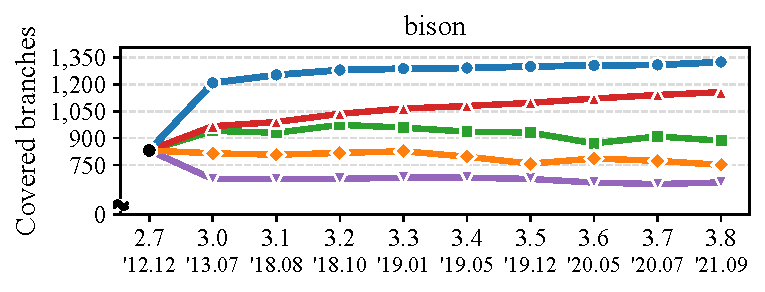
\includegraphics[clip, trim={0.25cm 0.33cm 0.22cm 0.25cm}, width=0.32\linewidth]{figures/fig_2_bison_lines.pdf} &
        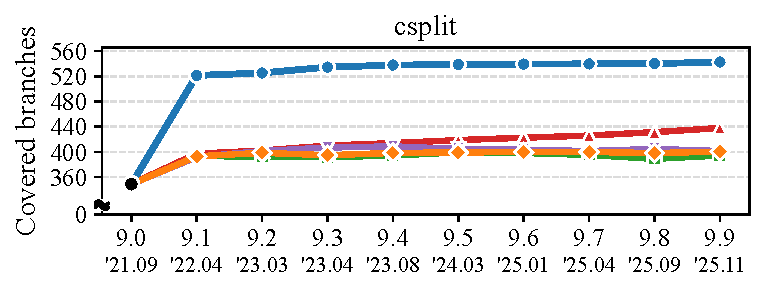
\includegraphics[clip, trim={0.25cm 0.33cm 0.22cm 0.25cm}, width=0.32\linewidth]{figures/fig_2_csplit_lines.pdf} &
        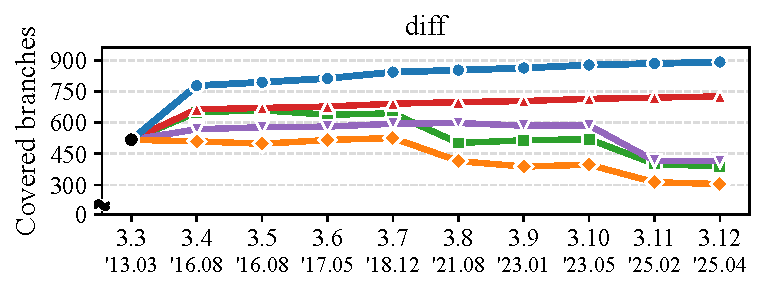
\includegraphics[clip, trim={0.25cm 0.33cm 0.22cm 0.25cm}, width=0.32\linewidth]{figures/fig_2_diff_lines.pdf} \\
        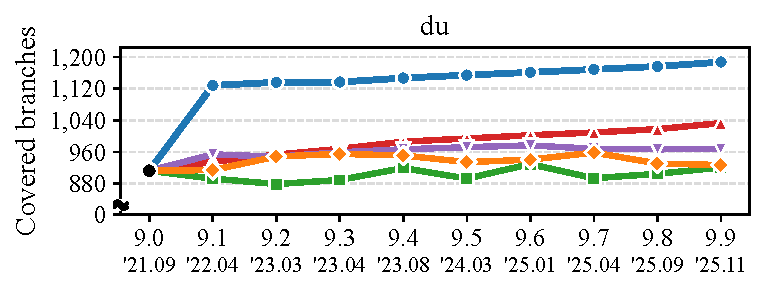
\includegraphics[clip, trim={0.25cm 0.33cm 0.22cm 0.25cm}, width=0.32\linewidth]{figures/fig_2_du_lines.pdf} &
        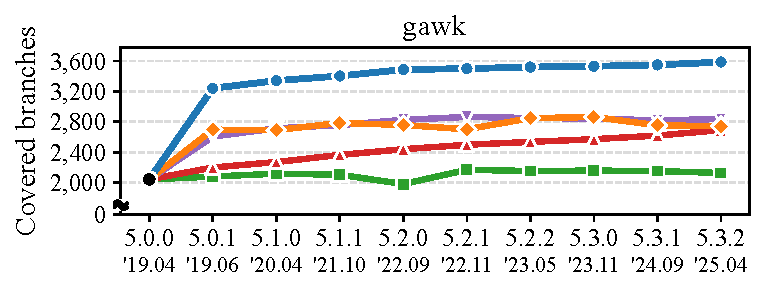
\includegraphics[clip, trim={0.25cm 0.33cm 0.22cm 0.25cm}, width=0.32\linewidth]{figures/fig_2_gawk_lines.pdf} & 
        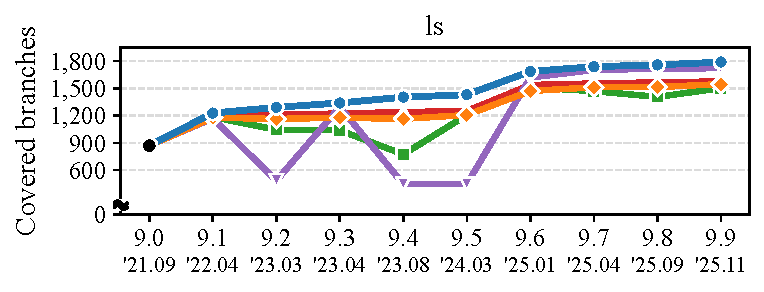
\includegraphics[clip, trim={0.25cm 0.33cm 0.22cm 0.25cm}, width=0.32\linewidth]{figures/fig_2_ls_lines.pdf} \\
        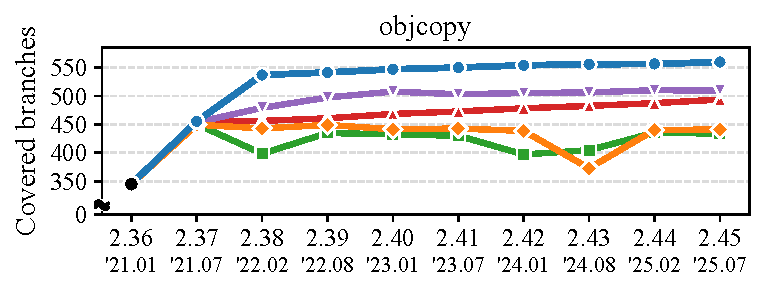
\includegraphics[clip, trim={0.25cm 0.33cm 0.22cm 0.25cm}, width=0.32\linewidth]{figures/fig_2_objcopy_lines.pdf} &
        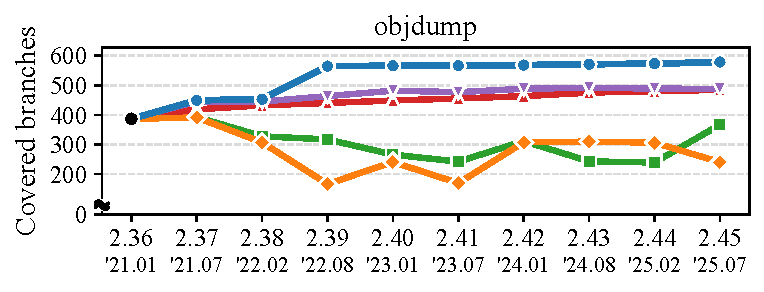
\includegraphics[clip, trim={0.25cm 0.33cm 0.22cm 0.25cm}, width=0.32\linewidth]{figures/fig_2_objdump_lines.pdf} & 
        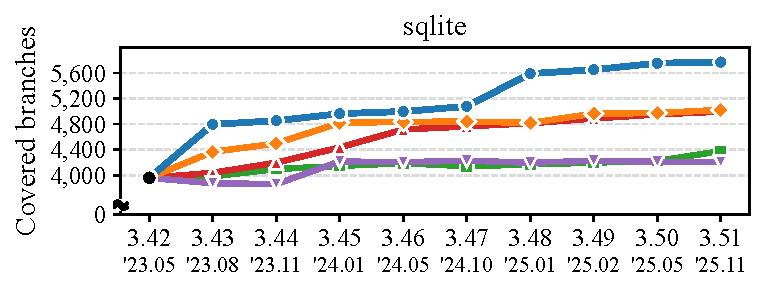
\includegraphics[clip, trim={0.25cm 0.33cm 0.22cm 0.25cm}, width=0.32\linewidth]{figures/fig_2_sqlite_lines.pdf} \\
        \multicolumn{3}{c}{
\includegraphics[clip, trim={0.0cm 0.15cm 0.0cm 0.05cm}, width=0.5\linewidth]{figures/fig_2_legend_small_cap.pdf}}
    \end{tabular}%
    }
    \caption{Branch coverage changes across ten consecutive releases of nine actively updated benchmarks.}
    \label{fig:long_coverage}
\end{figure*}

\myparagraph{\bf Multi-Release Efficiency}
To evaluate the efficiency of $\ourtool$ over more releases, we extended the experiment to ten releases and compared $\ourtool$ against the baselines. Specifically, from Table~\ref{tab:benchmarks}, we selected 9 actively maintained programs whose average update interval is less than one year. This allows our evaluation to cover release histories spanning up to 12.1 years between the first and last releases.

Figure~\ref{fig:long_coverage} shows that $\ourtool$ maintains higher coverage across all releases. On average, $\ourtool$ covered 28.2\% more branches than the four baselines across the nine subsequent releases: 37.5\% more than $\default$, 20.5\% more than $\rerun$, 30.0\% more than $\seeding$, and 24.7\% more than $\naive$. The performance gap between $\ourtool$ and the baselines grew as testing proceeded across releases. $\ourtool$ achieved 22.5\% higher branch coverage on average when testing the second release, and this improvement increased to 31.5\% for the last release. In particular, the performance gap between $\ourtool$ and $\naive$ increased the most, rising from 17.8\% to 31.1\%. 
% Statistically, the p-value against the baselines steadily decreased from 0.082 in second-release testing to 0.021 in last-release testing, suggesting that the improvements become increasingly significant across releases. 
These results highlight that $\ourtool$ effectively refines query data accumulated across releases and continuously improves the performance of subsequent-release testing.